\documentclass[12pt]{report}
\usepackage{graphicx,amssymb,amsmath,amsthm,ctable,booktabs,graphics}
\usepackage[colorlinks]{hyperref}
\usepackage[all]{hypcap} 
\usepackage{gensymb}
\usepackage{xcolor}
\usepackage{savetrees}
\usepackage{caption,subcaption}
%\renewcommand{\familydefault}{\sfdefault}
\usepackage[english]{babel}
%\usepackage[T1]{fontenc}
%\usepackage{helvet}
\usepackage{multicol}
\usepackage[utf8x]{inputenc}

\renewcommand{\sectionautorefname}{\S} %for \autoref
\renewcommand{\subsectionautorefname}{\S} %for \autoref
\renewcommand{\subsubsectionautorefname}{\S} %for \autoref

\newcommand{\ty}[1]{\textcolor{teal}{\texttt{#1}}}
\begin{document}

\title{Gemini-South IFU Data Reduction User Manual}
\author{Elaine M. Snyder\\
Dept. of Physics \& Astronomy\\
University of North Carolina at Chapel Hill \\
\texttt{emsnyder@live.unc.edu}}
\date{February 22, 2016}
\maketitle

\hypersetup{linkcolor=magenta}
\tableofcontents
\listoffigures
\begingroup
\let\clearpage\relax
\listoftables
\endgroup

%\begin{multicols*}{2}

\chapter{Introduction}
Greetings, Gemini Multi-Object Spectrograph (GMOS) integral field unit (IFU) data reduction pipeline user! Before beginning your data reduction journey, it will be important to understand the structure of an IFU and the way the Gemini IFU data is stored in the fits files you'll be reducing. If you are familiar with this already, feel free to skip ahead. Most of this information can be found online on \url{https://www.gemini.edu}, but I've compiled it all here for easy reference and so that I may reference it in the context of the RESOLVE\footnote{\url{http://www.resolve.astro.unc.edu}} survey's instrument setups.

\section{What is an IFU and why would we want to use one?}
\label{ifu}
The basic idea of any spectrograph is that incoming light from an object goes through a slit, is dispersed by a grating/prism/grism, and then focused onto your detector to create an image of your spectrum. Most of the time the slit is long and narrow ($\sim0.5-2''$ typically), and most astronomers would align it along a galaxy's major axis. This image will thus has spectral information in the x direction and spatial information in the y direction. The GMOS IFU is different in that instead of having one slit aligned along a galaxy's major axis, you will have multiple fibers that cover the entire galaxy. These fibers act as ``mini slits'', and each one will be dispersed and refocused onto the detector. This means you receive spectral information from all parts of the galaxy, not just where a single slit falls, and therefore are getting x, y, and wavelength at once. Thus, the main benefit of using an IFU is that it enables the 3D spatial analysis of the kinematics, metallicities, or whatever else you may want to derive from your spectra.

In the case of the GMOS IFU setups for RESOLVE observations, you will have either 750 or 1500 hexagonal fibers (depending on which setup was used) that cover an on-sky area of $5''\times3.5''$ or $7''\times5''$. See the top portion of \autoref{figure:1}, which shows the positions of the fibers over an example galaxy. As \autoref{figure:1} shows, the GMOS IFU is designed in such a way that not all of the fibers are centered on the object -- either 250 or 500 of the fibers are positioned on a region of sky away from the target (but not too far away), which enables the sky level to be later subtracted during data reduction. The sky level can be affected by moon illumination, clouds, etc. so it is important to be able to subtract any extra sky light there may be. Note that sometimes in online documents, the fibers may be called ``spaxels'', which is short for ``spectral pixels'' -- don't be confused by this hip IFU lingo.

\begin{figure}[h]
\centering
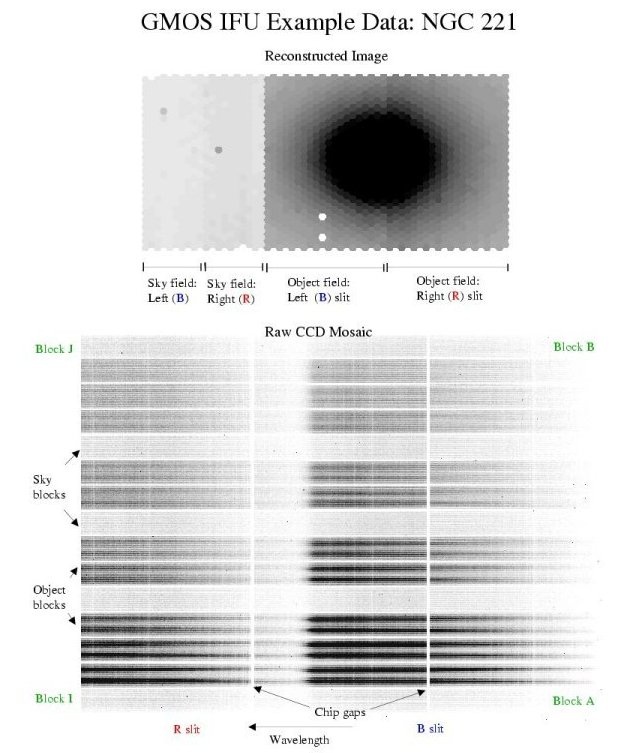
\includegraphics[width=0.8\textwidth]{fiber_examples.jpeg}
\caption[IFU Fibers and Data Format]{The top part of this image shows the IFU field of view over NGC221 (not a part of RESOLVE). The left portion of the image shows the sky spaxels, and the right portion shows the light of the galaxy. This is a 2D representation of the data we are getting -- the third dimension is in the wavelength direction, and the darkness over where the galaxy is from summing the light inside each spaxel there. The bottom portion of this image shows the raw fits data from the above galaxies.  \footnotesize{Image from \url{https://www.gemini.edu/sciops/instruments/gmos/spectroscopy/integral-field-spectroscopy/field-slit-mapping}}}
\label{figure:1}
\end{figure}

\section{Observing setups}
\label{setups}
As alluded to before, there are two main setups for RESOLVE's IFU observations. Similarly to our SOAR observations, there is a blue setup for absorption line galaxies and red setup for emission line galaxies. \autoref{table:1} highlights the main differences between the two setups. To determine which galaxy is best for which setup, we ideally like to use the SOAR broad spectrum as a guide. Seeing strong emission in the broad spectrum will point to the emission line setup on Gemini being best, while no emission will point to the absorption line setup being preferred. However, since there is not always a SOAR (or even an SDSS) spectrum available, we often rely on their photometric colors as an indicator of whether emission or absorption is more likely.

Using the GMOS IFU is ideal for RESOLVE's purposes for two different reasons. In the red setup, our goal is to obtain velocity fields for RESOLVE's smallest emission line galaxies. Thus, the spatial information we receive from the IFU spectra is ideal for this purpose. On the other hand, for the blue setup, our goal is to derive velocity dispersions. The small, absorption line galaxies we target with the IFU in the blue setup are often quite faint, so instead of focusing on the spatial information the IFU gives, we sum all the spaxels out to the effective radius of the galaxy, thereby summing the light enough to derive accurate dispersion measurements. 

We estimate exposure times for both setups using the online Integration Time Calculators\footnote{\url{http://www.gemini.edu/node/10479}} (ITC) supplied by Gemini. We use an elliptical galaxy SED template for time estimates in the blue setup and adjust our exposure time calculations so that we may achieve a signal-to-noise ratio of 25 per \AA\ when we bin all the fibers out to the effective radius of the galaxy. We use a model H$\alpha$ line with estimates of the line flux and continuum flux density for time estimates in the red setup, and adjust our exposure times to achieve a centroiding accuracy of $\sim5.3$ km s$^{-1}$. For both setups, we bin our spectra by 2 in the spectral direction to increase the signal-to-noise as well.

We also use the ITC to select central wavelength positions that ensure our features of interest do not fall in a chip gap (see bottom of \autoref{figure:1}). We choose two different central wavelengths so that we can fill in the chip gaps as well when we sum the individual exposures -- this is sometimes referred to as ``spectal dithering''. The central wavelength positions selected for our setups are listed in \autoref{table:1}.

\begin{table}
\centering
\begin{tabular}[t]{ccc}
  \hline
quantity  & blue setup & red setup \\ \hline
wavelength range & 4200 -- 5600 \AA\ &  5500 -- 6900 \AA\ \\ 
used for & absorption line galaxies & emission line galaxies \\
central wavelengths & 4850, 4900 \AA\ & 6300, 6400 \AA\ \\
features of interest & H$\beta$, Mgb, Fe5270, Fe5335 & H$\alpha$, [NII], NaD \\ 
grating & B1200 & B600 \\ 
filter & none (open) & r-G0326 \\
slits & 1 slit & 2 slits \\ 
field of view & $3.5''\times5''$ & $5''\times7''$ \\ \hline
\end{tabular}
\caption[RESOLVE's Observation Setups]{Comparison of RESOLVE's red and blue observation setups for the Gemini-South IFU.}
\label{table:1}
\end{table}

\section{Observing patterns}
\label{patterns}
In 2-slit (aka red setup) mode, we oftentimes will tile the IFU field of view in order to cover the entire extent of the galaxy. The $5''\times7''$ field of view can either be tiled to $10''\times7''$ for larger, rounder galaxies or to  $5''\times14''$ for longer, skinnier galaxies. This doesn't make a large difference to the reduction routine, but there will be more science frames to reduce and more data cubes to stack at the end.

The basic observation sequence is different for each mode. Both will start with acquisition images to ensure the IFU field of view is centered on the galaxy. Then flats, arcs, and science frames are taken in each dither. For example, a flat, arc, science, and arc frame will be taken at one central wavelegth, and then an arc, science, arc, flat frame will be taken at the other central wavelength, in that order. For reduction, we will want to flat field and wavelength transform the science images using the arcs and flats taken in the same dither. Once the data cubes are made, we can then sum the data cubes, both spatially and spectrally.

\section{Files you'll need for reduction}
\label{files}

The fits files you'll want for your data reduction can all be found online in the Gemini Science Archive (\url{http://archive.gemini.edu}. You will have to create an account with your unique observing program ID and program key (usually sent in an email for each new semester). RESOLVE's IDs are GS-2013B-Q-51 for the fall 2013 semester, GS-2014B-Q-13 and GS-2014B-Q-52 for the fall 2014 semester, and GS-2015B-C-1 (and carry-over GS-2014B-Q-13 band 1 time) for the fall 2015 semester (email Elaine or Sheila\footnote{\url{sheila[at]physics[dot]unc[dot]edu}}, if you need the program keys for any of these programs). Once your account is created, you can look at each observing program and download the data you want.

As alluded to \autoref{patterns}, you'll have flats, arcs, and science data for each galaxy in each wavelength dither. Normally, there are 2 flats, 2 or 4 arcs, and 2 or 4 science frames, depending on the estimated exposure times and/or the spatial offsets needed.

We also obtain a suite of baseline standards each semester -- one standard for both the red and blue setups that will be used for each galaxy observation taken that semester. This includes a science observation of standard star along with flats, arcs, and twilight flats in both wavelength dithers. We use the twilight flats to create response functions for each fiber in the IFU, and use the standard star science observations to correctly flux calibrate our galaxy data.

Lastly, we'll want a bias image in order to perform the bias subtraction. Each night after observing is complete, a standard set of bias frames are observed by the Gemini South operators. They are a little tricky to find in the online database, but you can go to the ``View Associated Calibrations'' tab to find all of the biases taken. Usually, searching on the observation date, the correct binning (CCDSUM 2 1), and the correct filter (see \autoref{table:1}) will yield 5 bias frames to download and process with the Gemini IRAF routine, gbias. I have downloaded these already for the RESOLVE data, and have trimmed, overscan subtracted, and stacked them.

\section{How the data is stored}
\subsection{The raw fits files}

Simply opening one of the S....fits files with DS9 will yield a strange result. You'll see a very long and skinny image appear. What you are actually seeing is 1/12th of the full image. This is because there are 3 CCDs and each one has 4 individual amplifiers that are read out into different extensions in your fits file. To see all the extensions, type \ty{ds9 -mecube S....fits}, which will open a cube dialog box that lets you scroll through each extension in the file. See \autoref{fig:mecube} and \autoref{fig:rawflat} as an example of what you'll see when you open a raw image. A part of the data reduction is to mosaic all of these extensions onto one single large image.

\begin{figure}[h]
\centering
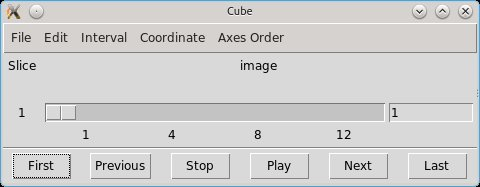
\includegraphics{mecube_raw.jpeg}
\caption[Example of DS9 cube diaglog box]{This is an example of the cube box that will open when you load a raw image in DS9.}
\label{fig:mecube}
\end{figure}

\begin{figure}[h]
\centering
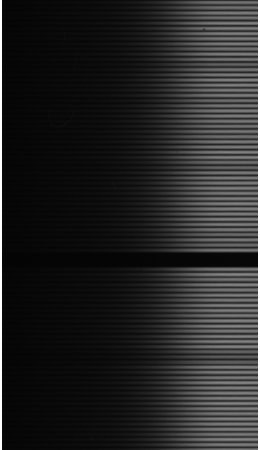
\includegraphics{raw_flat.jpeg}
\caption[Example of DS9 cube diaglog box]{This is an example raw image. Specifically this is a flat image, but you can also open the raw science and arcs. Each row you see is a fiber, and in the x direction is wavelength.}
\label{fig:rawflat}
\end{figure}

\subsection{What is an MDF?}
The mask definition file (MDF) stores important information about the image and is ``attached'' to the raw images as one of the first steps in the data reduction process. The actual file is in binary fits format and comes with the Gemini IRAF package. It is called either ``gsifu\_slitr\_mdf.fits'' or ``gsifu\_slits\_mdf.fits'' for the 1- and 2-slit data, respectively. The information stored includes the x and y spatial positions of each fiber number, as well as which fibers are good and bad. As a part of the data reduction, you will inspect and number each fiber, and if you find a fiber that is bad, but is not marked as bad in the MDF, you will have to edit the MDF manually. If this happens, email Elaine since the pipeline assumes the default MDF is fine.

\chapter{Setting Up Your Workspace}

There are some things you'll need to install (or update) before using this pipeline. I highly recommend working in the Ureka environment, which includes easy-to-install versions of IRAF, Python, and PyRAF. Since this code is written for PyRAF, Ureka is indeed quite handy. Instructions on how to download Ureka can be found here: \url{http://ssb.stsci.edu/ureka/}. I am currently using version 1.5.1 on cielo. Follow the instructions for making IRAF, and check your login screen to make sure it says you're using IRAF 2.16:

\begin{verbatim}
> pyraf

NOAO/IRAF PC-IRAF Revision 2.16 EXPORT Thu May 24 15:41:17 MST 2012
  This is the EXPORT version of IRAF V2.16 supporting PC systems.
\end{verbatim}

There is also an updated IRAF Gemini package you'll want to install. This version is not included in the Ureka download, but includes some updated tasks you will be using. Here's the link to this newest version as of February 2016: \url{https://www.gemini.edu/?q=node/11823}. You'll also want to check this when you're done by loading the `gemini' package in IRAF:

\begin{verbatim}
--> gemini

     +------------------- Gemini IRAF Package -------------------+
     |             Version 1.13.1, December 7, 2015              |
     |             Requires IRAF v2.14.1 or greater              |
     |              Tested with Ureka IRAF v2.16                 |
     |             Gemini Observatory, Hilo, Hawaii              |
     |    Please use the help desk for submission of questions   |
     |  http://www.gemini.edu/sciops/helpdesk/helpdeskIndex.html |
     +-----------------------------------------------------------+
\end{verbatim}

This pipeline also makes use of a PyRAF script called PyFU which was written by James Turner, a support scientist at Gemini. The code will align and sum the data cubes we make during the reduction process. The package is available at the Gemini Data Reduction Forum (\url{http://drforum.gemini.edu/topic/pyfu-datacube-mosaicking-package/}), and comes with instructions on how to install and point to the package from your login.cl file.

You may also need to download L.A.Cosmic, an algorithm that finds and removes cosmic rays. You can read more about it at \url{http://www.astro.yale.edu/dokkum/lacosmic/}. You can download the IRAF spectroscopic version from that website, and will need to add a line in your login.cl: ``task lacos\_spec = /path/to/where/you/put/it/lacos\_spec.cl''. The pipeline will call this task during the cosmic ray removal step.

(For future, may add Voronoi binning algorithm download, too.)

If you are new to data reduction in general, you will want to download DS9, an astronomical imaging application that you'll use to view our data as you progess through the pipeline. Download DS9 from this site: \url{http://ds9.si.edu/site/Home.html}.

Next, you'll want data to actually reduce! You should have flats, arcs, science frames, and a bias image before getting started. You should also have response flats from the baseline twilights and a flux calibration from the standard star data. See \autoref{files} for more info on how to get your data and on each specific file you'll need. There should also be an observing log to inspect (RESOLVE data has obslog.txt or just log.txt) as well as an alternative line list file ``smalllinelist.dat'' that will be helpful during the wavelength calibration steps. Place all of these files in the same folder, since that's where the pipeline looks for them. 

Lastly, you'll want to download the actual pipeline. You can access the code and this handy user guide at \url{https://github.com/emsnyder/geminiDRpipeline}. Always be on the lookout for updates in the future! You can place the code anywhere you like, but a nice folder structure would be to have individual folders for each galaxy with the pipeline code a level above. Now you should be all set, congrats!

\chapter{Data Reduction Guide}

\section{Entering and Exiting the Pipeline}
Here are the basic start up commands: 
\begin{enumerate}
\item cd to the directory where you put your data
\item enter the Ureka environment by typing \ty{ur\_setup} in the command line 
\item enter PyRAF by typing \ty{pyraf} in the command line
\item open a DS9 window by typing \ty{!ds9 \&} at the prompt
\item enter the pipeline by typing \ty{execfile(`/path/to/your/code/gemreductionpipeline.py')}
\end{enumerate}

\noindent To end your session:
\begin{enumerate}
\item type \ty{CTRL-C} to exit the pipeline, if not out already
\item enter \ty{.exit} to exit PyRAF
\item use \ty{ur\_forget} to exit the Ureka environment
\end{enumerate}

\section{Organizing and Identifying Your Data}

\noindent The first thing the pipeline does is look in your folder and identify which files are there. It will print out the files it found and whether there are arcs/flats/science/etc. It is good to check this against your observing log! If you find mistakes, please email Elaine, since the pipeline doesn't have a way to let you manually fix IDs yet. Every files is identified by looking in the image headers, so problems here most likely will be missing images. If these all look correct, type \ty{1} to go on.

\section{Reduction of the Flats}

This very first step is often (in the author's experience) the most time-consuming and frustrating step of the entire reduction. We use the flats not only for flat fielding the science data, but also to identify the fibers as a reference for all the other files.

The package used here is a main part of the Gemini IRAF package and is called `gfreduce'. It has many different options, but for the flat, we are just going to attach the MDF file, do a bias subtraction, overscan subtraction, and fiber ID so that we may extract all the spectra.

\begin{figure}[h]
\centering
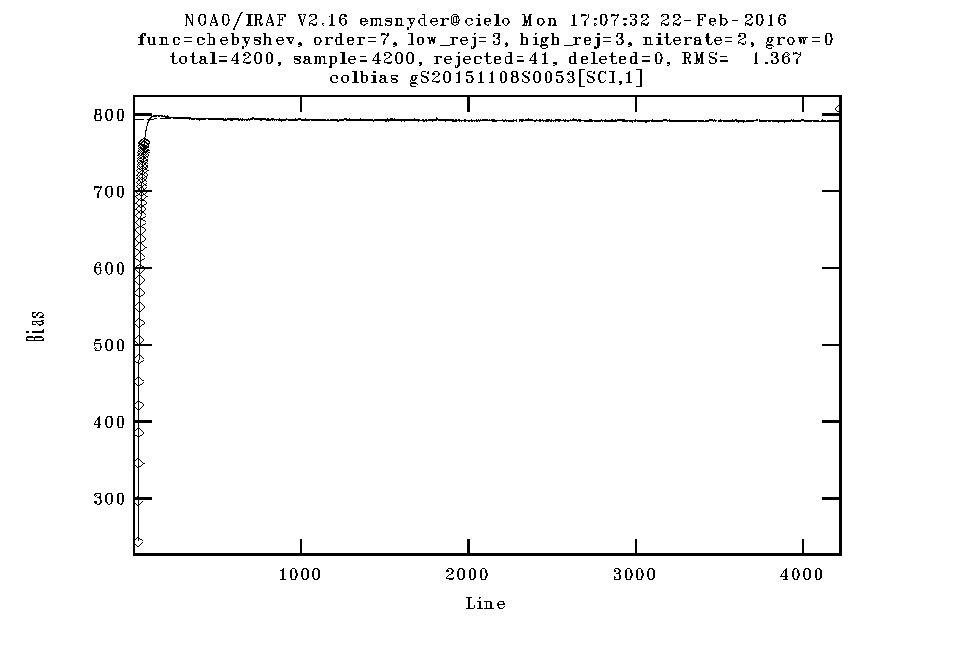
\includegraphics{overscan_example}
\caption[Overscan Subtraction Example]{An example of the overscan subtraction window that PyRAF will open during the reduction of the flats step. The solid line represents the data, while the dashed line shows the fit to that data. The diamonds are data points that are being rejected from our fit.}
\label{fig:overscan}
\end{figure}

\begin{enumerate}
\item The MDF attachment is done without user input needed. A file is produced in your working directory with the prefix `g'.
\item The bias and overscan subtraction is mostly done without user input needed. For the overscan subtraction, a PyRAF window will open with the overscan level being plotted.There is a also fit to the overscan level being plotting, and this normally looks fine as is. Press \ty{q} inside the PyRAF window to move on. There is a plot for each amplifier in the CCDs, so you will see 12 individual plots. If the fit does not look fine, you can type \ty{:order \#} and then \ty{f} inside the PyRAF window to change the order of the fit to a different number (with that number instead of \# in the previous command). Higher orders typically do better at fitting any strange features. Unless something is very wrong, you probably won't need to worry about this. See Figure \autoref{fig:overscan} for an example of what you should be seeing. This step produces a file with the prefix `rg', where the `g' comes from the previous step, i.e. the `rg' is both overscan and bias subtracted and has the MDF attached.
\item Lastly, we must tackle the fiber identification. Your command window is going to ask you a few questions:
\begin{verbatim}
Extracting slit 1
Find apertures for ergS20151108S0053_1? (`yes'): 
\end{verbatim}
Here I recommend saying `yes', as usually IRAF will be able to identify the fibers correctly for you. 
\begin{verbatim}
Edit apertures for ergS20151108S0053_1? (`yes'): 
\end{verbatim}
Say `yes' to this one as well, so we can inspect the fiber IDs and make sure everything looks correct. \autoref{fig:aps} shows what this will look like -- a complete mess! But we can zoom in by typing \ty{w} in the PyRAF window, and then typing \ty{e} at the bottom-left of the first `fiber bundle' and again at its top-right. [Note: use \ty{w} and \ty{a} to un-zoom the window.] You should now have a screen that looks like \autoref{fig:aps}. I find that making this plot full-screen helps immensely. Each `bundle' contains a set of 50 fibers, which you will see numbered at the top of your screen (though not very apparent in \autoref{fig:aps}). Your job is to make sure each fiber is identified correctly -- this means no repeated numbers or missing fibers. Often I find that the low level of fiber 50 makes it get skipped in IRAF's auto-finding scheme, which makes the first fiber of the second `bundle' start at 50 instead of 51. If this happens, you can use \ty{d} in the plot window to delete the IDs for fibers 50--750, and then use \ty{m} to re-mark the fibers. This is where it can get frustrating! \\

Figure \autoref{fig:bad} shows an example of a bad fiber not being marked in the identification process. This is exactly what we want to happen in this case. If you find another fiber that looks bad, you will have to edit the MDF file to `turn off' that fiber number. For the 2014-2015B slit-1 data, you will end with either fiber 742 or 743 (the rest up to 750 are bad). \\

If you are pleased with your IDs, type \ty{q}. More questions will appear in the terminal, but it will want your answer inside the PyRAF graphics window.

\begin{verbatim}
Trace apertures for ergS20151108S0053_1? 
\end{verbatim}

\ty{yes}

\begin{verbatim}
Fit traced positions for ergS20151108S0053_1 interactively?
\end{verbatim}

\ty{NO} (the capitals will tell IRAF no to all)

\begin{verbatim}
Write apertures for ergS20151108S0053_1 to database
\end{verbatim}

\ty{yes}

\begin{verbatim}
Extract aperture spectra for ergS20151108S0053_1?
\end{verbatim}

\ty{yes}

\begin{verbatim}
Review extracted spectra from ergS20151108S0053_1?
\end{verbatim}

\ty{NO}

If you're in the blue setup (1-slit mode), this is the end of IDing for you! If you're in the red setup (2-slit mode), you'll have to repeat this process for fibers 751--1500 (usually fibers 1493 and above are missing for this group). Once complete, IRAF will extract all the spectra and create a file with the prefix `e', so in full you should have an `ergS....fits' file in your working directory. Since we have two different wavelength dithers, you'll have to repeat this process for the second flat, but after that, we'll use these files to identify the fibers for the rest of the bunch.

\end{enumerate}

\begin{figure}[t]
\centering
\begin{subfigure}[t]{0.49\textwidth}
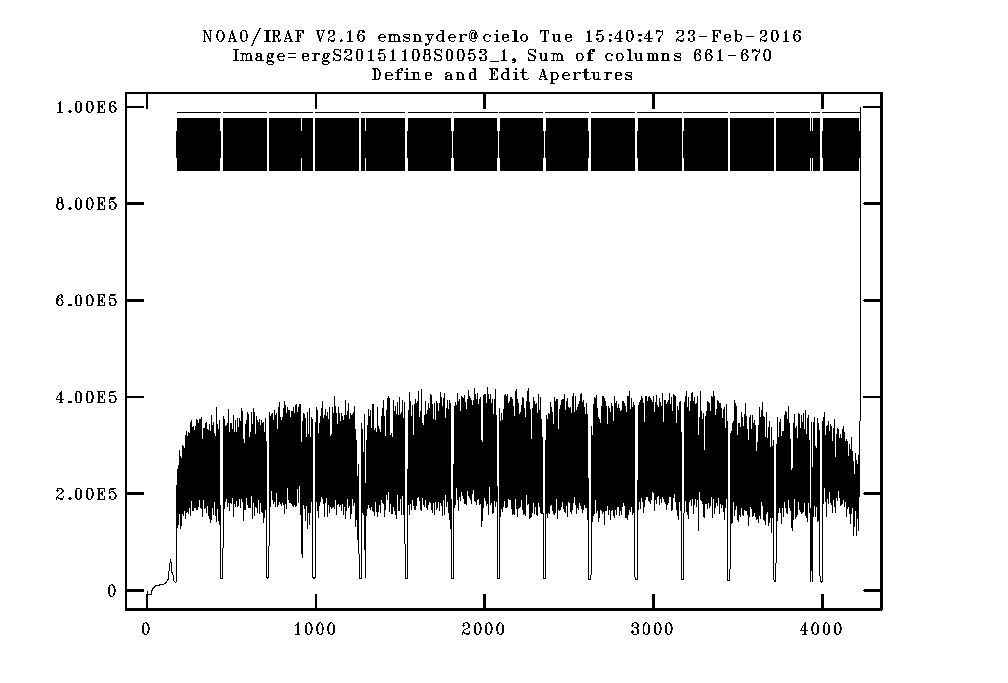
\includegraphics[width=\textwidth]{apertures1}
\end{subfigure}
\hfill
\begin{subfigure}[t]{0.49\textwidth}
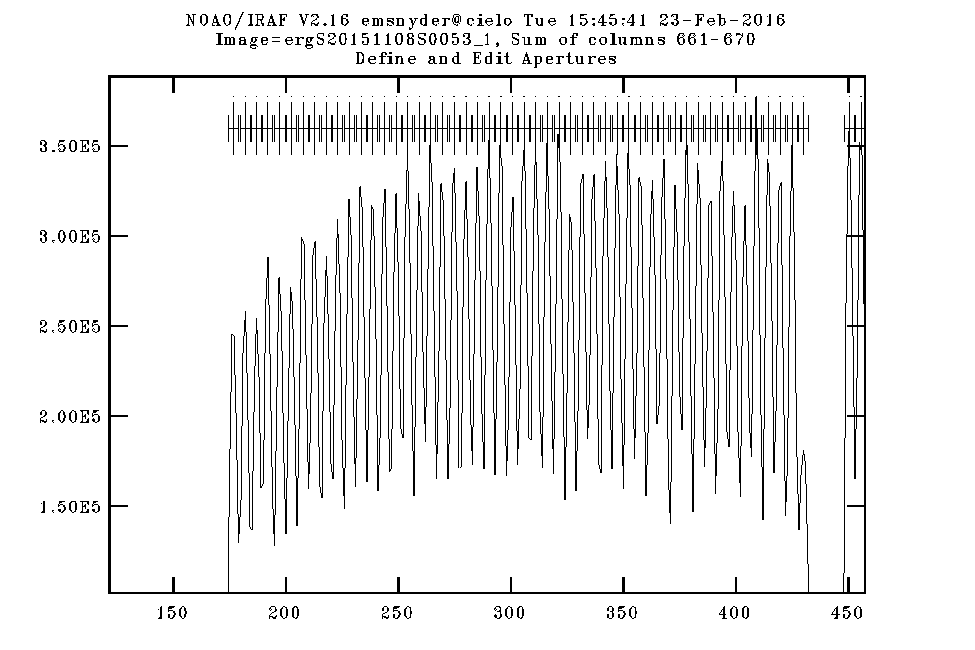
\includegraphics[width=\textwidth]{apertures2}
\end{subfigure}
\caption[Examples of the Fiber ID Step]{\textbf{(a).} A zoomed-out example of the fiber ID window that PyRAF will open during the reduction of the flats step. \textbf{(b).} An example of the fiber ID window that is zoomed-in on one set of fiber bundles.}
\label{fig:aps}
\end{figure}

\begin{figure}[h]
\centering
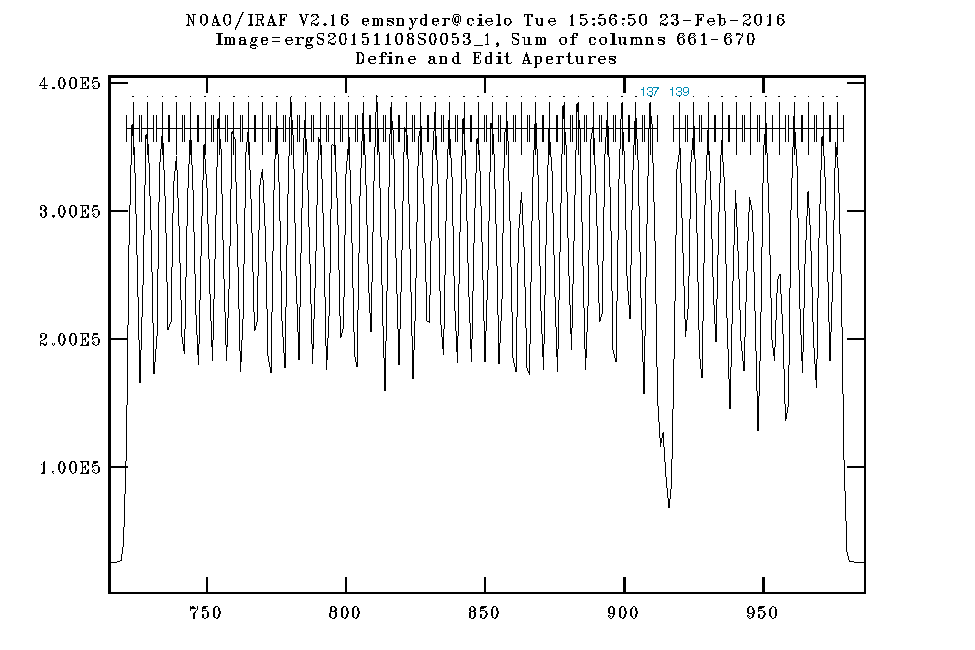
\includegraphics[scale=0.8]{badfiber}
\caption[Example Image of a Bad Fiber]{For this image, fiber 138 is bad. The MDF knows this though, and that number is skipped during the identification routine.}
\label{fig:bad}
\end{figure}


\section{Overscan Subtraction of the Arcs}

The next step is to add the MDF and overscan subtract the arcs. A bias subtraction isn't needed here since the arcs are read out ``faster'' than the bias frames. There is nothing interactive for this step.

\section{Identification and Removal of Bad Pixels from the Flats and Arcs}
\label{badpix}

\begin{figure}[h]
\centering
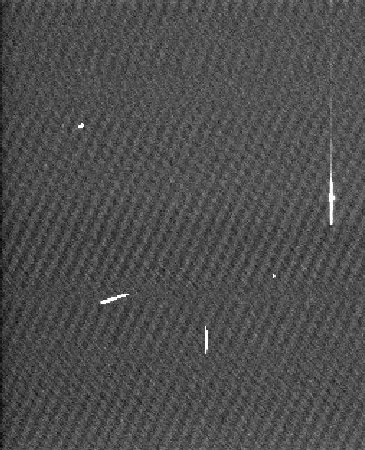
\includegraphics[scale=0.8]{CRvsBP.jpeg}
\caption[Cosmic Rays vs. Bad Pixels]{This image shows you both cosmic rays and bad pixels. The long line on the right side is a bad column, whereas the other three bright spots are probably cosmic rays.}
\label{fig:badpix}
\end{figure}

Before we get too into the reduction, we must look at our bias-subtracted images and find any hot pixels that could later affect the reduction. The bad pixels may be different for images taken at different exposure times, so we'll need to create a bad pixel map (BPM) for the flat, arc, and science frames separately (though the separate dithers can use the same BPM).

The pipeline will open a DS9 window with one of the flats first. It will then prompt you to look through all twelve extensions and identify any bad pixels or columns you see. If you don't see any bad pixels, you can enter \ty{0} and move on to the arcs. If you do see some bad areas, enter \ty{1}, which will bring up another prompt for you to enter the extension number, and x and y values of the bad region. The extension number can be 1-12, and x and y can extend to the full size of your image. To enter a bad rectangle, you can say x = 132:140 and y = 444:450. For a full column, you can enter * for y.

It is important to discern between cosmic rays and bad pixels too. I usually find that cosmic rays will be curved and erratic looking, while actual bad pixels will be in straight lines and will be much larger. See \autoref{badpix} for examples. Generally, you'll have the same bad areas in all images, but the extent of the damage due to these pixels can vary due to exposure time. So, if you're unsure of a bad pixel vs. cosmic ray, look in the other images to see if there's any there. We will clean the cosmic rays from the science data in a separate step. You will repeat this for an arc image, and later in the reduction will do this for the science frames as well.

\section{Extraction of the Arcs}

This step will use the fiber IDs you created from the flat images to extract the spectra from the arcs. There is nothing interactive for this step.

\section{Creation of the Wavelength Solution}
\label{waves}

Next, a PyRAF window will open and you will see an image that looks like \autoref{fig:wave}. With the smaller line list that was included in your downloads, only $\sim 15$ will be chosen automatically. Press \ty{f} to see the fit residuals, which should look something like \autoref{fig:resids}. The number we want to pay attention to here is the RMS. I try to keep this under $\sim0.09$\AA, which, after some experimenting, I've found produces a good wavelength solution. You can also change the order of the fit using \ty{order: \#}. This default order is 4, which seems to work well most of the time. 

At times, especially when going from slit 1 to slit 2, the first line on the left will be misidentified. You can delete lines with \ty{d} and then re-identify them by hovering your mouse above the correct line, typing \ty{m}, and then entering the correct wavelength. Refitting with \ty{f} should then yield a better RMS value.

\begin{figure}[h]
\centering
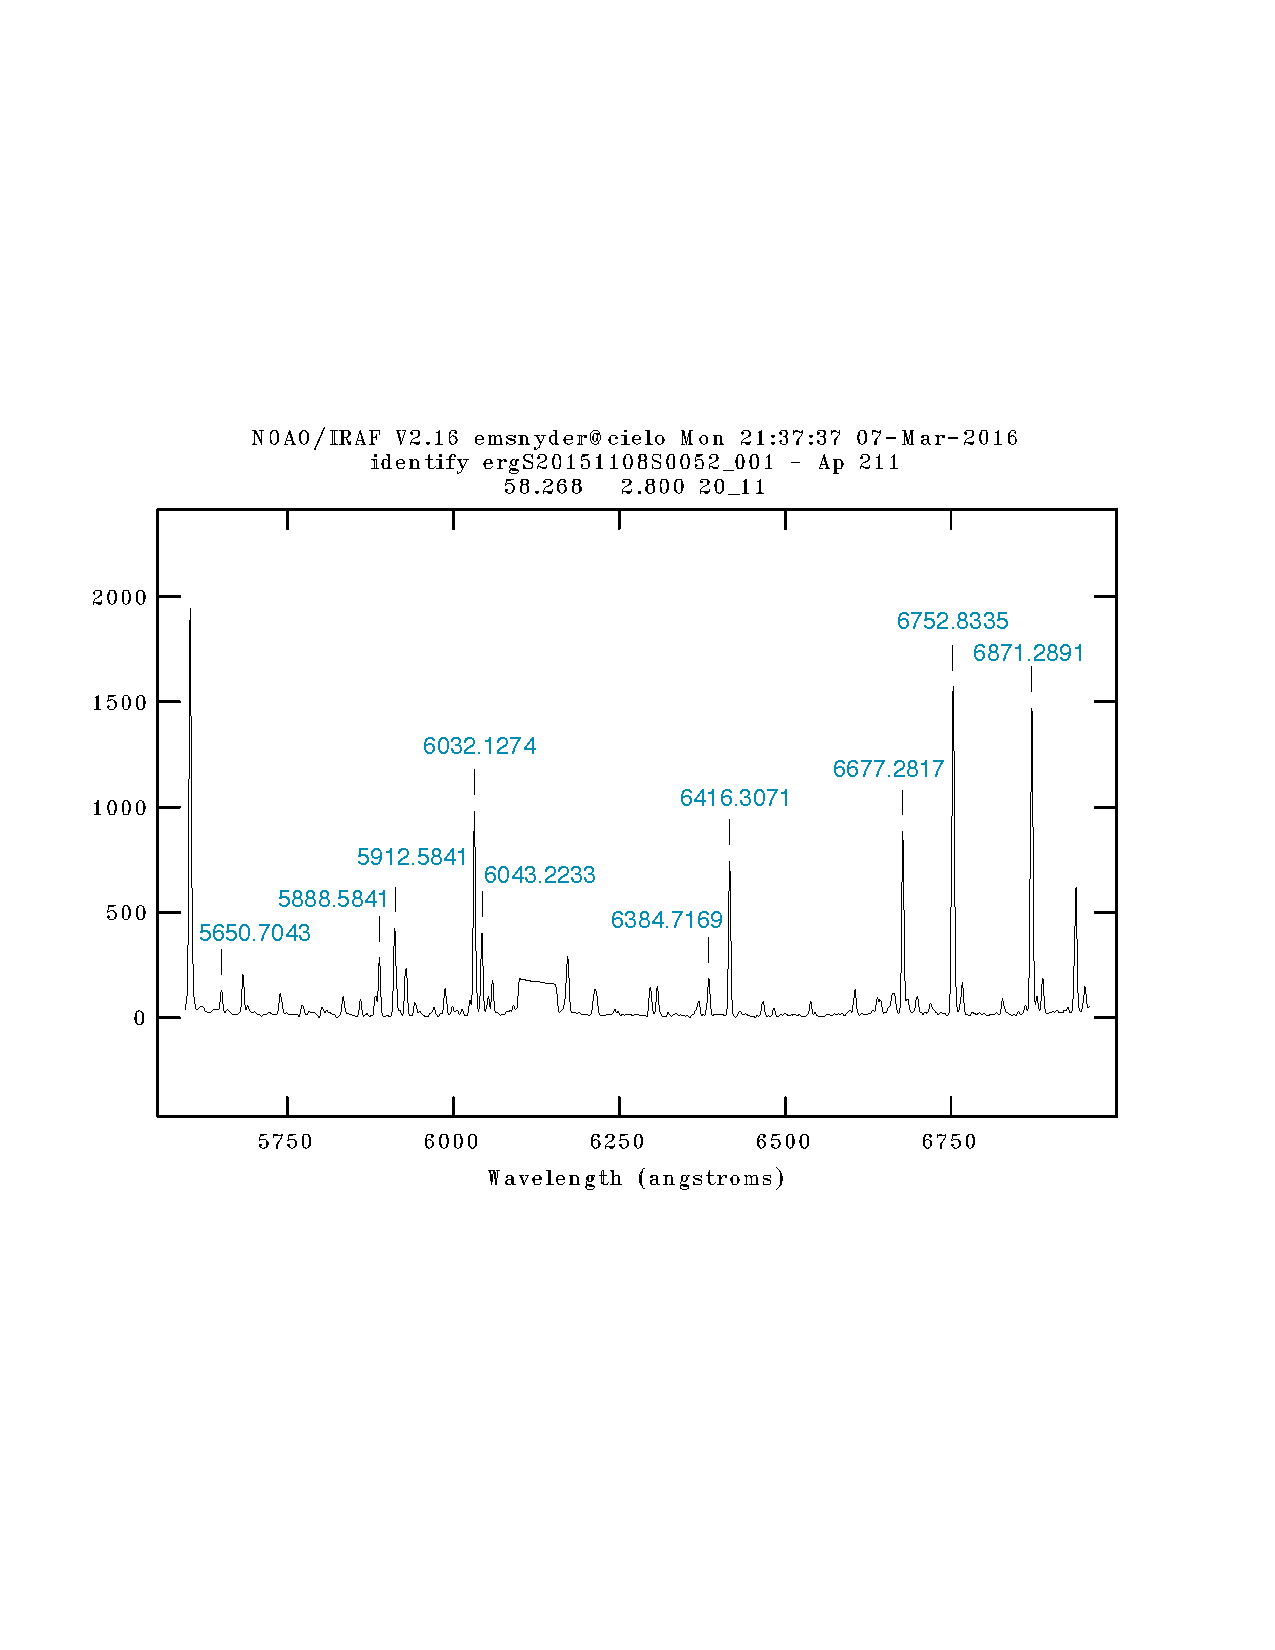
\includegraphics[scale=0.6]{wavelength_example_new}
\caption[Example of the wavelength solution]{This image shows the arc spectrum in one of the fibers. The arc lamps have certain emission lines that will appear, and we know the wavelengths of those lines automatically. This lets us create a function that assigns a wavelength to all of our image pixels.}
\label{fig:wave}
\end{figure}

\begin{figure}[h]
\centering
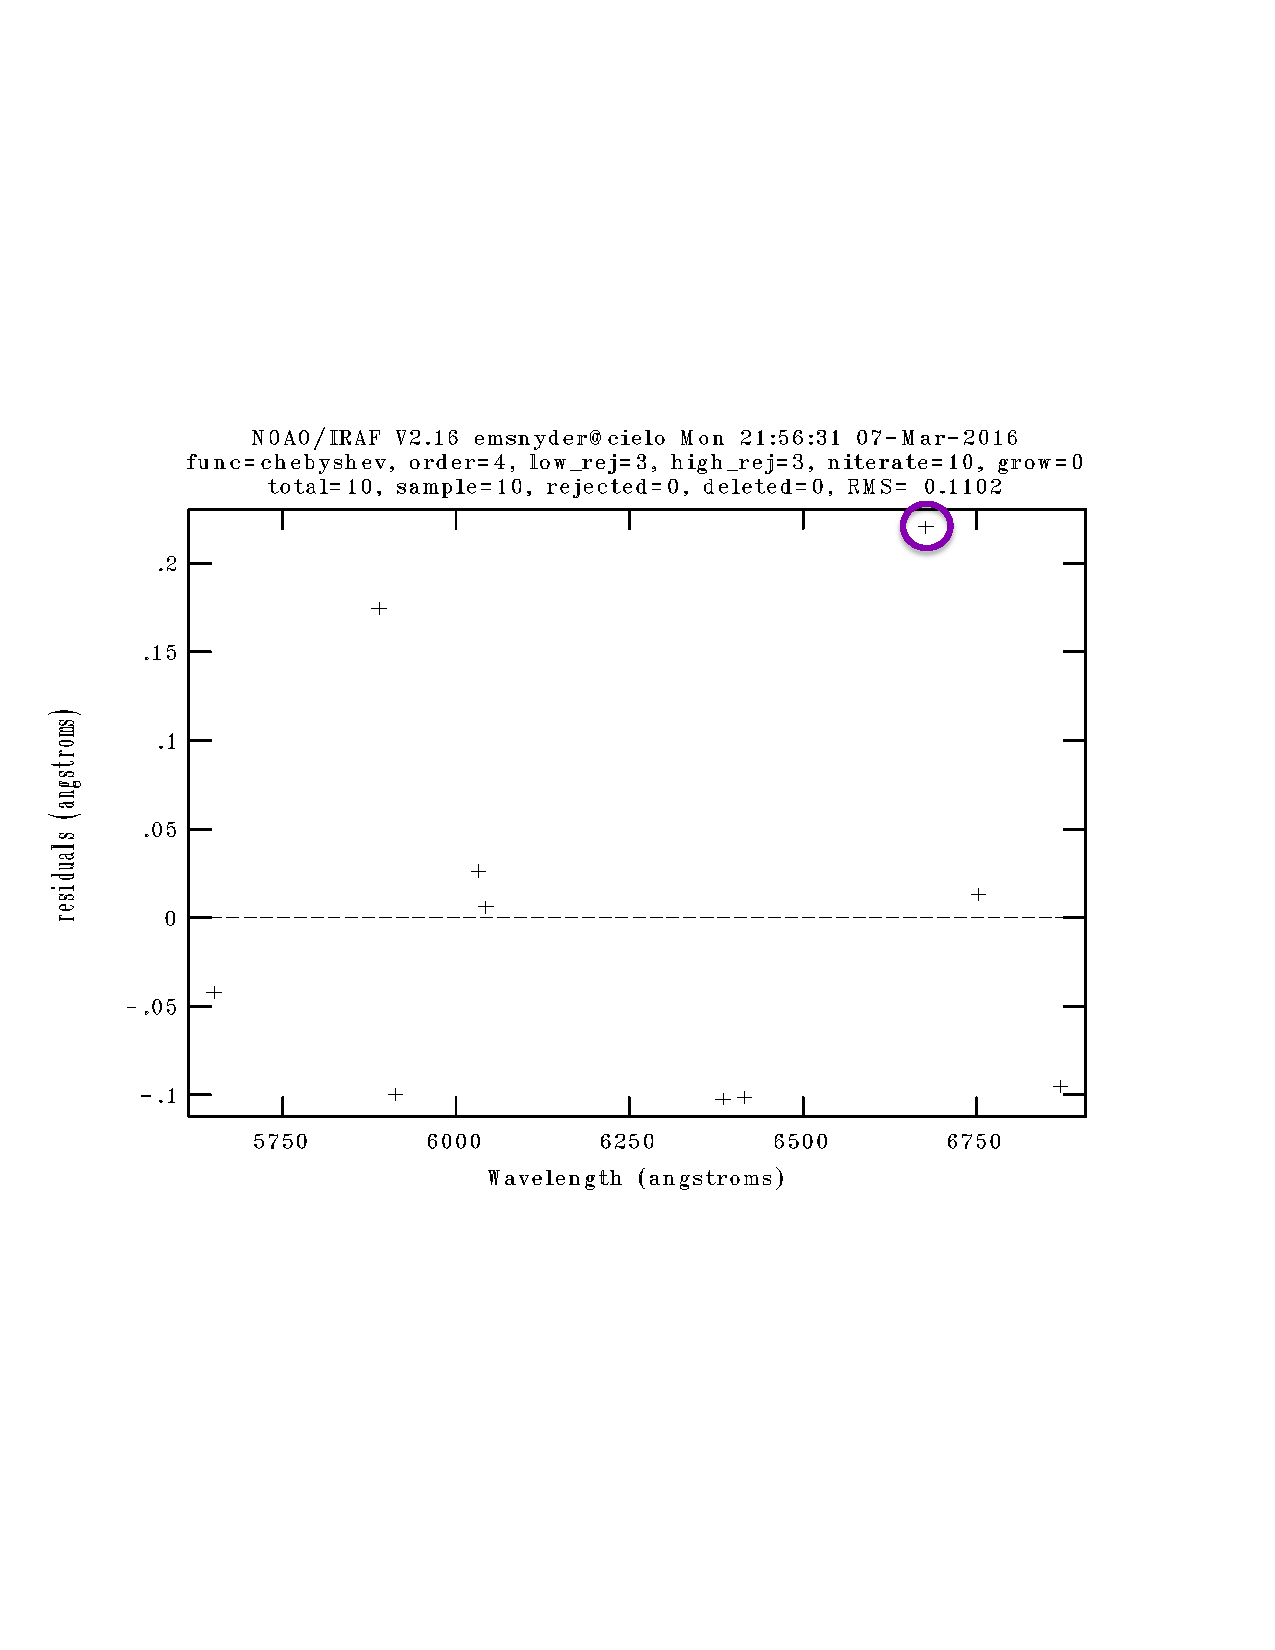
\includegraphics[scale=0.6]{wave_red_bad_new}
\caption[Example of the residuals of the wavelength fit]{This image shows the residuals of the wavelength function fit.  To improve this fit, I would delete, using \ty{d}, the circled point. You can also change the order of the fit if the default (4) doesn't fit well enough.}
\label{fig:resids}
\end{figure}

You will see on your PyRAF screen some text that looks like this:

\begin{verbatim}
          Image Data    Found          Fit   Pix Shift    User Shift Z Shift      RMS
ergS20151108S0106_001 - Ap 440 10/10   10/10   -0.00557     0.00522  1.82E-6   0.0749
Fit dispersion function interactively? (no|yes|NO|YES) (`no'): 
ergS20151108S0106_001 - Ap 441 10/10   10/10    -0.0793       0.081  1.36E-5   0.0731
Fit dispersion function interactively? (no|yes|NO|YES) (`no'): 
ergS20151108S0106_001 - Ap 442 10/10   10/10    -0.0694      0.0711  1.12E-5    0.034
Fit dispersion function interactively? (no|yes|NO|YES) (`no'): 
ergS20151108S0106_001 - Ap 443 10/10   10/10   -0.00833     0.00873  9.11E-7   0.0476
Fit dispersion function interactively? (no|yes|NO|YES) (`no'): 
ergS20151108S0106_001 - Ap 444 10/10   10/10     0.0222     -0.0225  -4.0E-6     0.07
Fit dispersion function interactively? (no|yes|NO|YES) (`no'): 
ergS20151108S0106_001 - Ap 445 10/10   10/10     0.0256     -0.0259  -4.7E-6   0.0896
Fit dispersion function interactively? (no|yes|NO|YES) (`no'): 
ergS20151108S0106_001 - Ap 446 10/10   10/10      0.084     -0.0855  -1.4E-5    0.126
Fit dispersion function interactively? (no|yes|NO|YES) (`no'): yes
\end{verbatim}

My way of conquering this task is to answer \ty{no} to each prompt until I see an RMS value that needs attention. For example, the last row in the above text is where I said yes to fit the wavelength function interactively when the RMS was 0.126. If the RMS is okay, I won't fit it interactively. You will need to do this for each fiber. The new output for this step are files in the database named ``idergS....\_001" and ``\_002'' (if in 2-slit mode).

\section{Application of the Calibration to the Arcs}

This step simply applies the wavelength solution you just found to the arc lamps itself. A good way to check our work here is to make sure the arc lines in the output image (which will start with the prefix ``terg") are straight, as opposed to curved. See Figure XX for a before and after. If everything looks good, we can use this same solution for our science data as well. If something looks wrong, an easy way to fix this is to delete the ID files created in the previous step, and start again. If you're in 2-slit mode and see that only one of the slits is bad, you can delete only the bad one of these files (either ``\_001'' for the first slit and ``\_002" for the second slit), and move the other one to a temporary file name. For example, if you find slit 2 is bad for one of the arcs, you can \ty{rm} IDergS...arc1\_002, and \ty{mv} IDergS...arc2\_001 to a temporary file name. Now you can restart the pipeline, go to the wavelength calibration step, answer \ty{NO} for slit 1 and redo the fits for slit 2. There will now be two new ID files, and you can replace IDergS...arc1\_001 with your temp file.

\begin{figure}[t]
\centering
\begin{subfigure}[t]{0.49\textwidth}
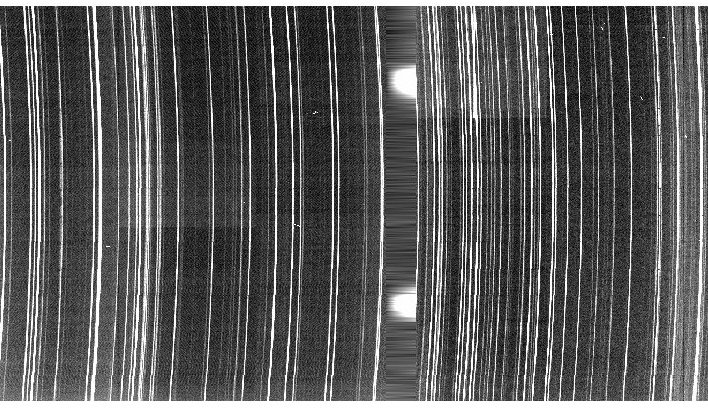
\includegraphics[width=\textwidth]{arc_before.jpeg}
\end{subfigure}
\hfill
\begin{subfigure}[t]{0.49\textwidth}
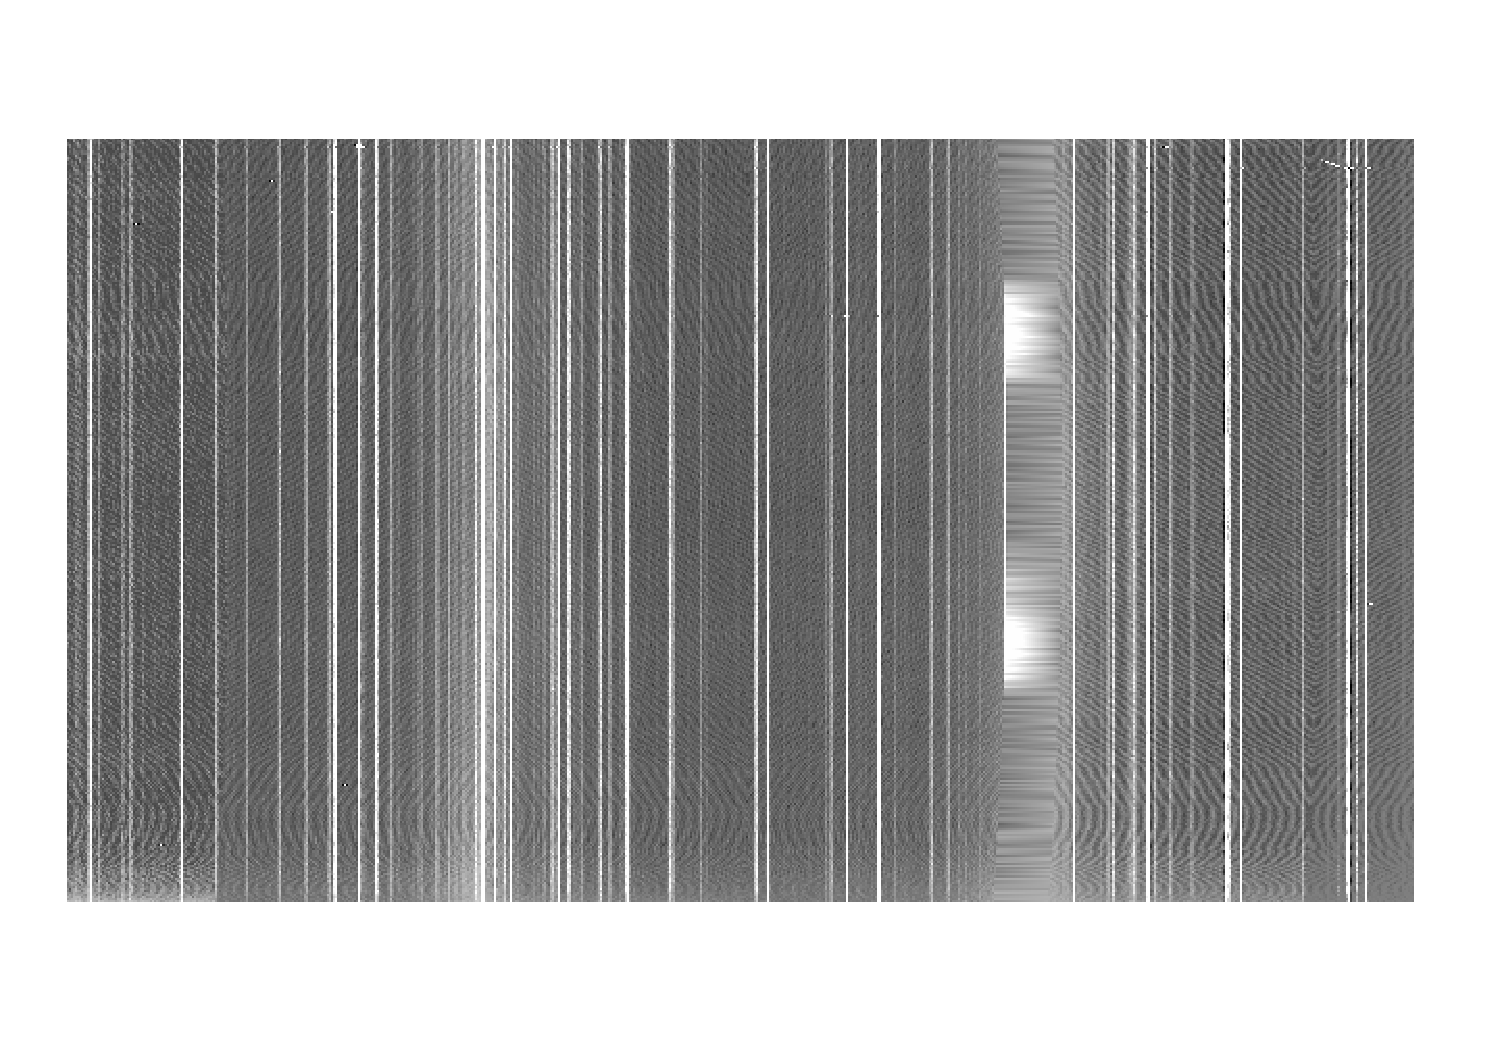
\includegraphics[width=\textwidth]{ds9}
\end{subfigure}
\caption[Before and After Wavelength Calibration]{\textbf{(a).} A DS9 view of the arc before the wavelength transformation has been applied. \textbf{(b).} The same, but after the wavelength transformation has been applied.}
\label{fig:skysub}
\end{figure}

\section{Quantum Efficiency Correction of Flats}
\label{qecorr}

Some CCDs will have different quantum efficiency levels between CCD sections or amplifiers, so this step corrects for this effect. Nothing interactive is required. This step creates files with the prefix `q'.

\section{Re-extraction of the Flats}

Now the flat spectra will be re-extracted, using the same fiber IDs as before, but this time pulling out the QE-corrected spectra. Again, nothing interactive must be done. After this step, our flats will have the prefix `eqprg'.

\section{Bias and Overscan Subtraction of Science Data}

Next, we perform the bias and overscan subtraction of the science frames. Nothing interactive is needed here.

\section{Identification and Removal of Bad Pixels from the Science Data}
We now make the BPM for the science data. See \autoref{badpix} for more information on this step. A file with the prefix ``p'' is made here.

\section{Cosmic Ray Rejection}

Next, we use L.A. Cosmic to find and remove cosmic rays from our science spectra. The code will iterate many times, and may take a few minutes to complete. Nothing interactive is required, and a file with the prefix `x' is created.

\section{QE Correction of Science}

We now QE correct the science frames, much like we did for the flats in \autoref{qecorr}. Again, nothing interactive is needed here, and you should have a file made with the prefixes ``qxprg".

\section{Flat Fielding and Extraction of Science}
Next, we use the response functions made from the twilights to flat field our science data, and then extract it. Nothing interactive is needed here, and a file with the prefix ``e'' is made.

\section{Wavelength Calibration of Science}
In this step, we apply the wavelength solution we found in \autoref{waves} to the science frames. There is nothing interactive for this step, and file is created with the prefix `t'.

\section{Sky Subtraction of Science}

Now, we can pull out the spectra of the sky fibers and use them to subtract the sky spectra from the science. A PyRAF window will open that looks like the left image in \autoref{fig:skysub}. The peaks that we see are probably cosmic rays that were not well subtracted, so if you hover your mouse near the peak and type \ty{d}, we can remove these artificial peaks. You can redraw the spectra after deleting using \ty{r}. When done, you should see an image like the right frame of \autoref{fig:skysub}. A file with the prefix ``s'' is made here.
\begin{figure}[t]
\centering
\begin{subfigure}[t]{0.49\textwidth}
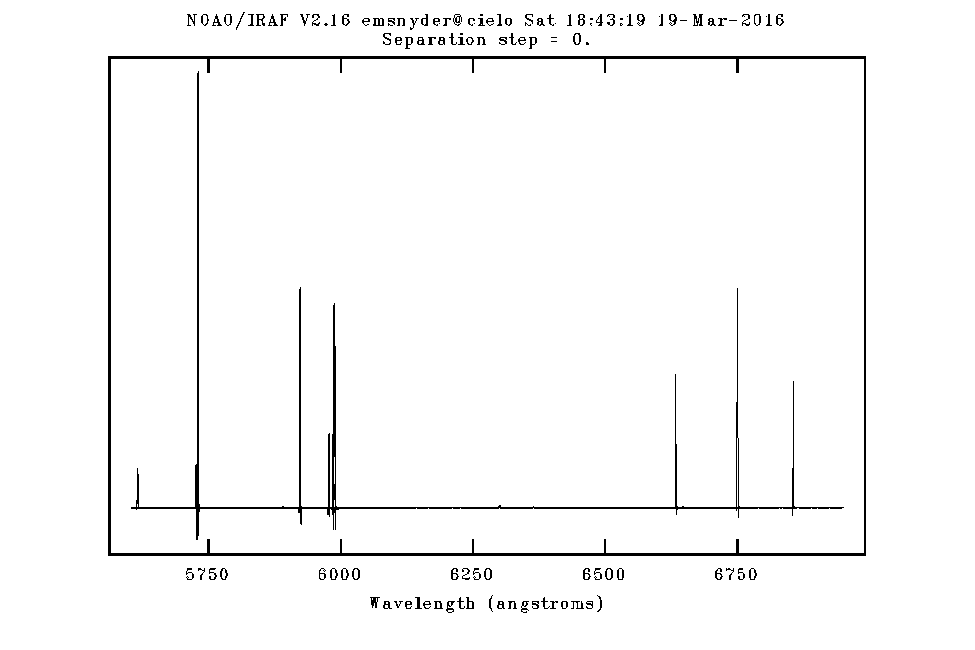
\includegraphics[width=\textwidth]{skysub_before}
\end{subfigure}
\hfill
\begin{subfigure}[t]{0.49\textwidth}
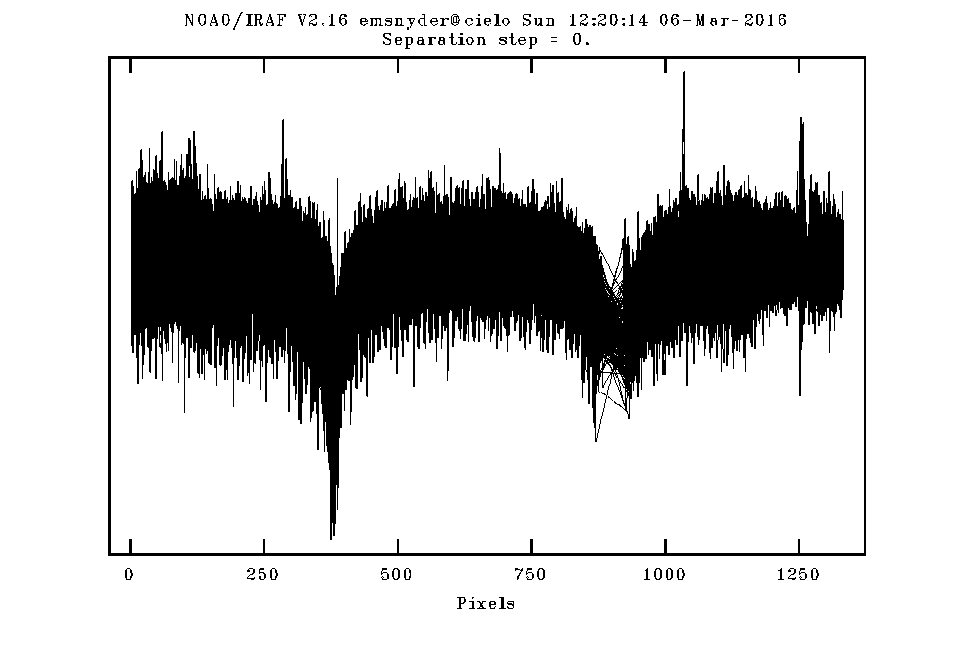
\includegraphics[width=\textwidth]{skysub_good_example}
\end{subfigure}
\caption[Examples of sky subtraction]{\textbf{(a).} An example of the sky subtraction PyRAF window you'll see initially. \textbf{(b).} An example of the remaining spectra after the peaks have been deleted.}
\label{fig:skysub}
\end{figure}

\section{Flux Calibration of Science}
The second to last step of the reduction uses the flux responses from the standard star data to flux calibrate our science data. Nothing interactive is needed here, and a file with the prefix ``c" is created.


\section{Data Cube Creation}
Now that we've reaching the end of the reduction process, we resample our spectra into data cubes. There will be as many data cubes as there are science images. We then sum the cubes in the spectral direction to fill the chip gaps and increase the signal to noise ratio. If there are spatial offsets, we can use the offsets in noted in the image headers to align and sum these as well. In the end, there is a final data cube for us to analyze. Files with the prefix ``d" are created here. Congratulations, you are done (for now)!


\chapter{Derivation of Kinematics}

\section{Deriving Velocity Dispersions}
\section{Deriving Rotation Curves}

%\end{multicols*}


\end{document}
